\documentclass[final,3p,sort&compress,12pt]{elsarticle}

%% The amssymb package provides various useful mathematical symbols
\usepackage{amssymb}
\usepackage{setspace}
\usepackage{pifont}
\usepackage{amsmath}
\usepackage{amsfonts}
\usepackage{pgf-pie}
\usepackage{pgfplots}
\usepackage{calc}
\usepackage{graphicx}
\usepackage{float}
\usepackage{anyfontsize}
\usepackage{pgfplots}
\usepackage{comment}
\usepackage{booktabs}
\usepackage{rotating}
\usepackage{siunitx}
\usepackage{eurosym}
\usepackage{multirow}
\usepackage{xcolor} 
\usepackage{colortbl}
\usepackage{subcaption}
\usepackage{blindtext}

\bibliographystyle{elsarticle-num-names} 

\DeclareSIUnit{\EUR}{\text{\euro}}
 \pgfplotsset{compat=1.17}


\journal{Energy and Buildings}

\begin{document}

\begin{frontmatter}

%% Title, authors and addresses

\title{Developing Decarbonisation Pathways for Irish homes in changing TIMES}


\author[inst1,inst2]{Jason Mc Guire \corref{j.mcguire@ucc.ie}}
\cortext[j.mcguire@ucc.ie]{j.mcguire@ucc.ie}

\affiliation[inst1]{organization={Energy Policy and Modelling Group, MaREI Centre},
            addressline={Environmental Research Institute}, 
            city={Cork},
            country={Ireland}}
            
\affiliation[inst2]{organization={School of Engineering},
            addressline={University College Cork}, 
            city={Cork},
            country={Ireland}}

\author[inst1,inst2]{Fionn Rogan}
\author[inst1,inst2]{Olexandr Balyk}
\author[inst1,inst2]{Tomás Mac Uidhir}
\author[inst1,inst2]{Ankita Gaur}
\author[inst1,inst2]{Brian Ó Gallachóir}
\author[inst1,inst2]{\& Hannah Daly}

 \onehalfspacing
\begin{abstract}
%% Text of abstract

Ireland has committed to one of the most ambitious decarbonisation targets in the world to 2030. The residential sector, responsible for 14.2\% of total greenhouse gas (GHG) emissions \cite{Howley2020Energy-RelatedIreland.} , is among the most carbon intensive per dwelling in the EU, emitting 60\% more $CO_2$ than the national EU average \cite{SustainableEnergyAuthorityofIreland2018EnergySector}, because of a high share of low thermal efficient detached dwellings coupled with a high dependency on carbon-intensive heating fuels. These factors have served as barriers to the decarbonisation of the residential sector in Ireland to date.  \par
Energy system optimization models (ESOMs) have been used extensively to inform pathways in addressing long-term energy challenges, which provides insights to decision-makers on issues related to climate and energy policy. \par
The TIMES-Ireland Model (TIM) is a newly developed optimisation model for the Irish energy system. This paper describes the methodology applied to the development of the residential sector in TIM and explores the results, which provides new insights on optimal residential decarbonisation pathways.

\vspace{0.25cm}
\noindent

\end{abstract}

\begin{keyword}

Energy Systems Optimisation Model \sep TIMES \sep Residential decarbonisation \sep Model description 

\end{keyword}

\end{frontmatter}

%% \linenumbers
\newpage
%% main text
 \onehalfspacing
\section{Introduction}
\label{sec:Introduction}

The Introduction section of this paper reviews bottom-up residential models, which have high technological granularity accounting for the residential sector only and ESOMs which have a bottom-up or hybrid approach and includes all energy-related sectors. The hybrid approach combines bottom-up technological detail and top-down macroeconomic detail. The introduction also analyses Ireland's distinctive residential sector, climate targets, and current energy policy. 

 \onehalfspacing
\subsection{Energy Systems Optimisation Modelling and the Residential Sector}
\label{Intro:ESOM}

Economically optimal or least cost residential decarbonisation pathways are dynamic, with technological advancements in heating appliances being assisted by exponentially increasing computational capacity over time, combined with new low-carbon fuel alternatives and new heating technologies becoming available. ESOMs have a rich representation of existing and future technological variables such as efficiency, cost, and fuel, while also accounting for macroeconomic variables such as economic growth and the social discount rate. ESOMs supply enough energy to at least satisfy energy service demands so that the lights stay on, while also considering sectoral interconnections to explore future decarbonisation pathways. There are a number of widely used ESOMs, such as MESSAGE \cite{Messner1995Model-basedPlanning}, TIMES \cite{Loulou2016DocumentationI}, Balmorel \cite{Wiese2018BalmorelModel}, TEMOA \cite{Hunter2013ModelingTemoa} and OSeMOSYS \cite{Howells2011OSeMOSYS:Development.}. 

These models can be used to explore the residential sector in higher granularity. Different levels of disaggregation are applied to the residential sector in models and research by \citet{Natarajana2011ModellingApproach}  highlighted a common approach used by defining an average performance for a number of dwelling categories, and this approach was adopted here. To account for the heterogeneous mix of dwellings, each dwelling is categorised based on building type to better reflect the housing stock and provide building specfic insights. Some models also disaggregate the year of construction \cite{Ahern2013StateStock}, wall type \cite{Dineen2015ImprovedSource} and level of insulation \cite{Clinch2001Cost-benefitEfficiency}.

% Average dwellings -	Would it be worth having a paragraph early in this section that describes some relevant characteristics of the residential sector, e.g. very heterogeneous mix of dwelling types (hence the archetype approach), a slow turnover of building stock (hence challenge of very ambitious near term targets), a broad distinction between new and existing dwellings (former very efficient, latter often not efficient), different types of energy use (space heating, water heating, appliances), drivers of energy demand (weather, affluence, demographics), non-economic rationality of dwelling occupants (hence caution required with techno-economic modelling approaches)? This might help frame your review. - Fionn


The Integrated MARKAL-EFOM System (TIMES) has been extensively used in both the UK and Ireland, and there are several examples of using TIMES to focus on the residential sector. TIMES assumes perfect foresight to enable a least-cost solution to be calculated, but \textit{``in reality, the behaviours of consumers is not always economically rational"} \cite{Li2018IncorporatingModel}. In light of this,  \citet{Li2018IncorporatingModel} investigated the heating technology preference in the UK using UK TIMES Model (UKTM) by incorporating a Discrete Choice Model (DCM) to better reflect how homeowners choose heating technologies and thus correcting for error in the perfect foresight assumption. 

There is a rising tendency for ESOMs to focus on new building fabric \cite{Leibowicz2018OptimalServices,Dineen2011ModellingHeating} and retrofitting to thermally improve the existing residential stock \cite{Dineen2015ImprovedSource}. Another trend observed is the electrification of energy-related sectors \cite{Chiodi2013ModellingSystem}, while a focus on photovoltaic (PV) systems can be examined in parallel \cite{Marczinkowski2018ResidentialSystems}. Retrofitting and electrification are a fundamental part of residential decarbonisation in Ireland, and therefore play a central role in the development of the model described here. 
Furthermore, the new model includes technologies, which were not previously considered, one such technology is District Heating (DH), some initial studies have found it may be optimal to have 37\% of heat demand to be provided by DH in Ireland \cite{Thellufsen2019ImplementingIreland}, the full list of space and water heating technologies considered in the model can be found in \ref{sec:appendixA4}. The strength of an ESOM can be used to examine the sectoral interactions, one study by Hedegard and Münster \cite{Hedegaard2013InfluenceOperation} examined the interaction between heat pumps and wind generation investments in Denmark, the results find it is optimal to install air-to-water heat pumps in non-DH areas. 


\subsubsection{Ireland: Residential Modelling}
\label{Intro:ESOMIreland}

ESOMs have been used to optimise Ireland's entire energy system \cite{Chiodi2013ModellingSystem,Connolly2009DevelopingUniversity.}, however no Irish studies use ESOMs to solely explore the residential sector, as many models look across multiple sectors. However, two examples of Irish ESOMs focusing the residential sector in higher granularity are outlined below.

In 2014, \citet{Rogan2014LEAPsSystem} linked OSeMOYOS to the Long Range Energy Alternatives Planning system (LEAP), which is a scenario-based simulation modeling tool used to analysis energy policy in all sectors of the economy. The models were linked to explore specific energy efficiency policies in the residential and other sectors. Three scenarios were explored, namely, the reference scenario, energy efficiency scenario, and energy efficiency+ scenario. The reference scenario assumes that 300,000 existing dwellings will undergo a shallow retrofit from 2009 to 2020, and the results show that residential total energy consumption rose 6.7\% in 2020, compared to 2008. In the energy efficiency scenario, 800,000 residential dwellings are retrofitted between 2009 and 2020, combined with the effect of other policies such as building regulations and low energy lighting, resulting in a 9.9\% reduction of energy consumption in 2020, compared to the reference scenario. The energy efficiency+ scenario also allows for 800,000 residential dwellings to be retrofitting, but accounts for deeper retrofits. This results in an energy consumption reduction of 16.5\% in 2020, compared to the reference scenario. \citet{Rogan2014LEAPsSystem} discussed the barriers, obstacles to investment, split incentives, and information gaps which restrict energy efficiency improvements. The insights highlighted the importance for the policy to not only look at the number of retrofits, but also the depth of retrofit, as shown by the different results in the scenarios. The model also found considerable scope for energy savings to be made through improved building regulations. 

In 2018, \citet{Thellufsen2019ImplementingIreland} investigated the potential for the implementation of DH in both the commercial and residential sectors of Ireland. The paper analyses the $CO_2-80$ scenario ( 80\% $CO_2$ reduction in 2050, compared to 1990 ) with and without DH using the previous Irish TIMES model and EnergyPLAN. The previous version of Irish TIMES did not account for DH, so EnergyPLAN is used to investigate the operation and  feasibility of DH in Ireland. A sensitivity analysis was performed on investment costs, heat grid losses, and discount rates. In all cases, the inclusion of DH was found to be favourable. The results find the conversion of 37\% of the Irish heat demand to DH to be optimal. Both the TIMES model and climate target used in this study are superseded and the study did not include the future heat savings expected from retrofitting, nevertheless this study has provided insights on the potential of DH.

\par  The majority of previous modelling on the residential sector in Ireland has involved bottom-up residential sector models. These models have provided insights on the input data, methodology, and results, and some studies are outlined below.
\par In the first comprehensive analysis of the Irish residential sector, Clinch and Healy examined fuel poverty \cite{Healy2002FuelIreland}, excess winter mortality \cite{Clinch2000HousingMortality}, market failures \cite{Clinch2000DomesticFailure}, occupancy behaviour \cite{Clinch2001ModellingEfficiency}, social benefit \& cost \cite{Clinch2001Cost-benefitEfficiency}  and energy efficiency  \cite{Clinch2003ValuingModel,Clinch2001Cost-benefitEfficiency,Clinch2001ModellingEfficiency}. 

\par
In 2011,  \citet{Dineen2011ModellingHeating} developed a residential bottom-up model to assess the impacts of measures in Ireland's National Energy Efficiency Action Plan (NEEAP). The model focused on new buildings and examined the energy efficiency of space and water heating by examining technology and building fabric thermal efficiency.  %The paper acknowledges that retrofitting of existing stock will play a large role in meeting energy efficiency targets, however it is not examined, nor is the internal temperature effect on energy efficiency improvements. 
Later in 2015, \citet{Dineen2015ImprovedSource} built on previous work in examining new dwellings, by examining the energy savings potential of energy efficiency improvement measures of the existing dwelling stock. The Dwelling Energy Assessment Procedure (DEAP) model was used, this is the national tool for Building Energy Rating (BER) calculation. The BER filters from this study were updated and applied in the model developed here. \citet{Dineen2015ImprovedSource} performed and sensitivity analysis and found that there was a 7.5\% change in energy consumption for every 1$^{\circ}$C internal temperature shift. Concluding, BER standard assumptions are poor as they vastly overestimate dwelling energy consumption, the average internal temperature across the Irish dwelling stock may be closer to 18$^{\circ}$C than 21$^{\circ}$C.
\par In 2013, \citet{Ahern2013StateStock} investigated thermal retrofit measures of the existing detached, oil centrally heated, rural housing stock. %A base geometry according to age bands and thermal characteristics was created in the study. The default values used in some of the BER database variables where highlighted. For example, there are assumed U-values when the roof insulation thickness is unknown, this is based on age, but there are no U-values for uninsulated roofs despite a 2001 survey finding 18\% of detached housing in Ireland had no roof insulation. 
\citet{Ahern2013StateStock} found dwellings built post-2000 consume the greatest amount of energy (kWh/annum), due to their large floor area. Concluding that the majority of thermal energy efficiency progress in Irish dwellings is being offset. The model results show that thermal improvement measures resulted in a reduction of running costs and $CO_2$ emissions by an average of 65\% for houses constructed prior to 1979, compared to houses built in 1979 or after resulting in an average 26\% reduction in running costs and $CO_2$ emissions from retrofit measures. This study highlights the low hanging fruit of pre-1979 oil centrally heated, rural housing stock. 
\par The Archetype Dwelling Energy Model - SQL (ArDEM-SQL) was developed by \citet{Uidhir2020ImprovingDecisions} ArDEM-SQL converts the Irish BER public database into Microsoft SQL language and calculates the annual energy consumption for space/ water heating, and lighting using EN 13790:2004 to simulate the potential for improved energy efficiency gains within an existing retrofit program. Mac \citet{Uidhir2020ImprovingDecisions} examined the Better Energy Homes (BEH) retrofit grant scheme. 
%The five most common retrofit combinations were simulated for 9 distinct archetypes (3 BER energy rating groups, and 3 building types) and compared these to alternative retrofit combinations which delivered additional efficiency improvements. 
The results show that the alternative retrofit scenarios can achieve additional energy efficiency gains of up to 86\%, relative to the set of retrofit combinations actually delivered from the program. This shows the the type of retrofit(s) and archetype can have a large affect on the energy saved.   

\par Finally, the Sustainable Energy Authority of Ireland's (SEAI’s) National Energy Modelling Framework (NEMF) is a suite of modelling tools used for modelling the Irish energy system. The SEAI is Ireland's national energy authority and they play a key role in bridging the gap between grant/policy and consumer, by assisting consumers to reduce energy. The models listed are some of the models used within SEAI's NEMF to model the impact of incentives and opportunities created by specific policy instruments. 

\begin{enumerate}[1.]
\item {Core Structural Model of the Irish Economy (COSMO)  is a macro-economic model used by the Economic and Social Research Institute (ESRI) to create a baseline forecast of energy consumption by sector} \cite{Bergin2017COSMO:Ireland}
\item{PLEXOS is a power systems modeling tool used for electricity modeling and planning} \cite{2021PLEXOSExemplar}
\item{Energy-efficiency policy analysis tool informs the energy efficiency estimates} \cite{Scheer2015UnlockingOpportunity}
\begin{enumerate}[i.]
\item{Complementary to the Energy-efficiency policy analysis tool is the Consumer Choice Model which determines the attractiveness of energy efficiency finance options}\cite{SustainableEnergyAuthorityofIreland2017BehaviouralSector}
\end{enumerate}
\item{BioHEAT is a techno-economic simulation model of bioenergy and heat} \cite{Durusut2018BioHEAT:Sectors}
\end{enumerate}

The models described in this section include a range of national ESOMs and bottom-up residential models with varied objectives. The complexity of models has increased significantly in the last 20 years, in Ireland, the models started out in Microsoft Excel and switched to Microsoft SQL, with much higher computational power. The growing BER database is providing high data granularity input to Irish models. 
%The internal temperature is becoming more frequently analysed in Irish residential studies, a recurring theme is the wide range of internal temperatures which Dineen et al. \cite{Dineen2015ImprovedSource} found this assumption significantly changes the final residential energy consumption. 



\subsection{Case study for Ireland}
\label{Intro:IreRSD}

Ireland’s distinctive energy sectors are further separated from other EU member states when focusing on the residential sector. This is largely down to rural settlement patterns, larger dwellings, lower building thermal efficiency, and higher reliance on fossil fuels. This is illustrated by the fact only 5.8\% of the population of Ireland were living in apartments in 2018, the lowest in EU-27 and well below the 25.3\% average \cite{Eurostat2021DistributionSurveyilc_lvho01}, furthermore 71.4\% of the Irish population are deemed to be living in dwellings too large, where the EU-27 rate is 33\% \cite{Eurostat2021ShareSurveyilc_lvho50a}. The low thermal efficiency of Ireland's dwelling stock is highlighted by two facts; (i) 2021 building regulations require a 70\% reduction of $CO_2$ emissions in new dwellings compared to dwellings built in 2005 \cite{DepartmentofHousing2021Gov.ieBuildings}, and (ii) Central Statistics Office (CSO) data states approx. 85\% of residential buildings are 2005 or older. Additionally, Ireland's fossil fuel dependency is underpinned by home heating oil, which accounts for the largest share of fuel usage in the residential sector at 37\% \cite{SustainableEnergyAuthorityofIreland2018EnergySector}, of which all is imported \cite{OCleirigh2020EnergySEAI}.

In the last 30 years, the extraction of indigenous peat has declined and consequently peat consumption has halved, in 2018 peat accounted for 12.3\% of residential GHG emissions. GHG emissions from coal in the residential sector also declined to 6.9\% in 2018 \cite{Howley2020Energy-RelatedIreland.}. However, the decline in peat and coal has been offset by a more significant growth in oil in the same period, where oil accounted for 34.8\% of residential GHG emissions in 2018 \cite{Howley2020Energy-RelatedIreland.}. Despite being limited to some urban areas, gas still accounted for 15.5\% of residential GHG emission in 2018 \cite{Howley2020Energy-RelatedIreland.}. 
The residential sector relied on fossil fuels for over 90\% of thermal energy in 2018, consequently Ireland currently has the lowest renewable heat among EU member states, at only 6.3\% \cite{Eurostat2021ShareSourcesnrg_ind_ren}. %Preliminary results from the Environmental Protection Agency (EPA) have indicated a 9\% increase of residential GHG emissions in 2020, mainly due to low home heating oil prices and covid-related restrictions, proving some consumers are economically rational by filling oil tanks when prices are low. 

Space and water heating are the main energy services, accounting for 80\% of the energy used in residential dwellings \cite{SustainableEnergyAuthorityofIreland2018EnergySector} and typically have a lifetime of at least 15 years, consequently leading to a slow turnover of technology in the residential sector. Apart from space and water heating, all EU member states are required under commission regulation (EU) 431/2014 to supply energy consumption data on space cooling, cooking, lighting \& appliances, and others (mainly outdoor appliances), the annual trend of these energy services is shown in Figure \ref{fig:IrelandServiceDemands}. These energy services were also used in TIM, however there is no space cooling data available in Ireland and lighting \& appliances were separated while others was combined with appliances. 

% Space heating is the largest residential energy service, which accounted for 61.8\% of final energy usage in 2018. Other residential energy services and their share of final energy are shown in Fig.\ref{fig:Ireland2018ServiceDemands}. As building thermal efficiency and heating technology efficiency improves, both space and water heating energy would be expected to decline. 


\begin{figure}[!ht]
\centering
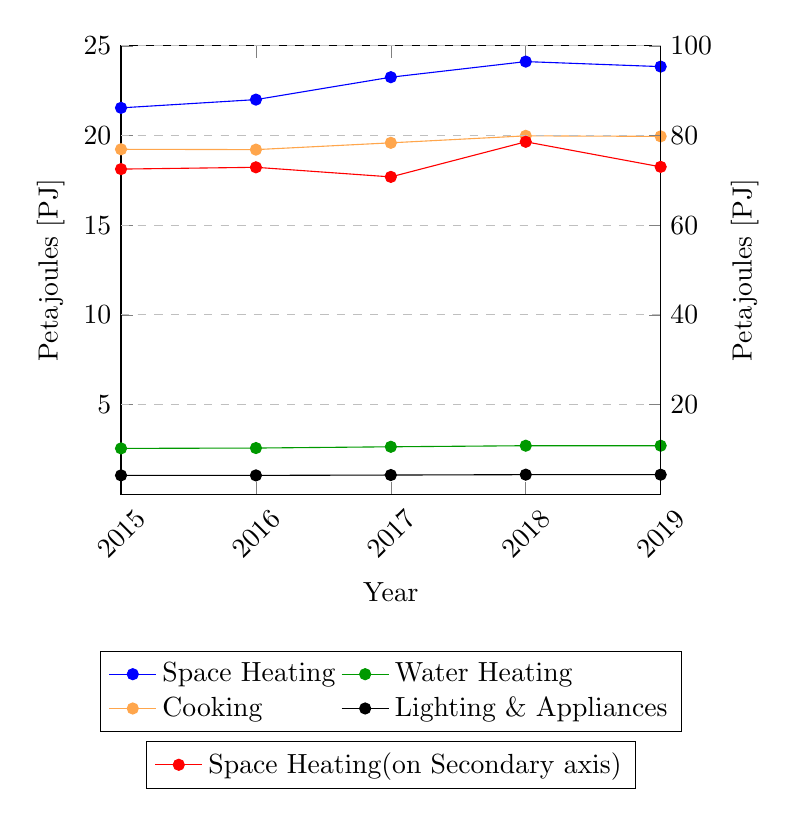
\begin{tikzpicture}
\begin{axis}[
    scale=1,
    legend cell align={left},
    x tick label style={/pgf/number format/1000 sep=,rotate=45},
    legend style={at={(0.5,-0.35)},anchor=north,legend columns=2},
    xlabel={Year},
    ylabel={Petajoules [PJ]},
    xmin=2015, xmax=2019,
    ymin=0, ymax=25,
    xtick={2015,2016,2017,2018,2019},
    ytick={5,10,15,20,25},
    ymajorgrids=true,
    grid style=dashed,
]

\addplot[
    color=blue,mark=oplus*
    ]
    coordinates {
    (2015,21.54)(2016,22)(2017,23.25)(2018,24.12)(2019,23.84)
    };
    
\addplot[
    color=green!60!black,mark=oplus*
    ]
    coordinates {
    (2015,2.55)(2016,2.57)(2017,2.64)(2018,2.7)(2019,2.7)
    };
\addplot[
    color=blue!60,orange!70, mark=oplus*
    ]
    coordinates {
    (2015,19.23)(2016,19.211)(2017,19.59)(2018,19.98)(2019,19.95)
    };
\addplot[
    color=black,mark=oplus*
    ]
    coordinates {
    (2015,1.046)(2016,1.045)(2017,1.065)(2018,1.086)(2019,1.084)
    };
    \legend{Space Heating,Water Heating,Cooking,Lighting \& Appliances, Other}
    
\end{axis}
%
\begin{axis}[
scale=1,
    scale=1,
    legend cell align={left},
    x tick label style={/pgf/number format/1000 sep=,rotate=45},
    legend style={at={(0.5,-0.55)},anchor=north,legend columns=2},
    xmin=2015, xmax=2019,
    ymin=0, ymax=100,
    xtick={2015,2016,2017,2018,2019},
    ytick={20,40,60,80,100},
    ymajorgrids=true,
    grid style=dashed,
    axis y line*=right,
    axis x line=none,
    ylabel style = {align=center},
    ylabel= {Petajoules [PJ]}
]

\addplot[
    color=red,mark=oplus*
    ]
    coordinates {
    (2015,72.5)(2016,72.9)(2017,70.76)(2018,78.59)(2019,73)
    };
    
     \legend{Space Heating(on Secondary axis)}
    \end{axis}
\end{tikzpicture}
\caption{Ireland Residential Energy Service Demands \cite{Eurostat2021Disaggregatednrg_d_hhq}}
\label{fig:IrelandServiceDemands}
  \end{figure}  


\subsubsection{Residential sector characteristics}
\label{Intro:GHG}

Under 2006 Intergovernmental Panel on Climate Change (IPCC) guidelines, Ireland’s residential sector accounted for 14.2\% of GHGs emissions in 2018 \cite{Howley2020Energy-RelatedIreland.}. Focusing only on energy-related GHG emissions from heat, electricity and transport, the residential sector directly accounts for 24\% of GHG emissions. The residential sector is directly responsible for 47\% of heat and 30\% of electricity and indirectly responsible for a share of the remaining GHGs, especially in the transport sector, as the rural settlement patterns increase transport demands. 

Under the Climate Action and Low Carbon Development (Amendment) Act 2021, the Irish government has adopted legally binding national targets to reduce GHG emissions by 51\% in 2030, compared to 2018. The Act also proposes a long-term target to achieve a climate neutral economy or ``net-zero" by 2050 \cite{2021Climate2021}. These targets account for all emissions - both Emission Trading System (ETS) emissions and non-ETS emissions, and sets out to make sectoral five-year carbon budgets a legal requirement to aid progress of the forementioned long-term targets. 
\par The EU's first Nationally Determined Contribution (NDC), which had a 40\% GHG reduction target (first NDC), has been succeeded by a new target of at least a 55\% GHG reduction target (updated NDC) by 2030 compared to 1990 levels. Ireland's Climate Action Plan 2019 (CAP2019) complies with the EU's first NDC, from which Irelands 30\% Non-ETS GHG reduction target in 2030 compared to 2005 levels was derived  \cite{DepartmentofCommunicationsClimateActionandEnvironment2019Climate2019}. Climate Action Plan 2021 will be more ambitious than its predecessor, CAP2019 as it must reflect EU's updated NDC target and take account of the national target also.
There are also renewable energy targets to consider for transport (RES-T), heat (RES-H), and electricity (RES-E) under the renewable directive (EU) 2018/2001, and the energy efficiency targets under (EU) 2018/2002.

\subsubsection{Policy context}
\label{Intro:Policy}
The Irish government's long-term overarching strategy aims to  achieve \textit{``effective density and consolidation, rather than more sprawl of urban development, [as] a top priority"}\cite{Ireland2018ProjectFramework}. The densification of Ireland's main cities will provide opportunities to improve the efficiency of heating, electricity, and transport within and between cities. 
\par The Marginal Abatement Cost Curve (MACC) produced in CAP2019, shows electricity \& transport are the most cost-effective sectors for energy decarbonisation \cite{DepartmentofCommunicationsClimateActionandEnvironment2019DecarbonisationIreland}. In Ireland, the decarbonisation of electricity is underway, with carbon intensity falling annually to 375 $gCO_2/kWh$ in 2018, which is 40\% lower than 2005 levels \cite{Howley2020Energy-RelatedIreland.}. 
Ireland uses both the \textit{carrot} (subsidy) and \textit{stick} (tax) approach to direct private investment towards low carbon or renewable energy. A €15/ $tCO_2$ carbon tax was introduced in 2009 to reduce investment in fossil fuels, and the increasing carbon tax rate has resulted in tax receipts growing every year from 2010 to 2018 \cite{Oireachtas2019AnOffice}. Ireland's current carbon tax of €33.50/ $tCO_2$ is set to rise to €100/ $tCO_2$ in 2030. The Renewable Energy Feed-in Tariff (REFIT) schemes were designed to incentivise renewable electricity investment to achieve legally binding renewable targets under 2009/28/EC. The Renewable Electricity Support Scheme (RESS) replaced REFIT in 2020. RESS supports renewable electricity projects to help Ireland achieve 2030 climate targets, especially the 70\% renewable electricity target. 

\par As the grant provider, SEAI plays a key role in the rollout of retrofitting and heat pumps. The retrofitting and heat pump grants do still require large upfront costs from the consumer, which may hinder the ambitious targets as this wont be a viable option for many households, green loans are currently available to bridge this gap. % are therefore the preferred heating technology despite the high capital costs. CAP2019 planned to retrofit 500,000 existing homes to at least a  ‘B2’ energy rating by 2030, which highlights the energy efficiency first approach in the residential sector. 
\par Gas Network Ireland (GNI) have set a 18\% biomethane target for 2030 \cite{Ervia2019VisionIreland}, where CAP2019 only set a 3\% biomethane target for 2030 \cite{DepartmentofCommunicationsClimateActionandEnvironment2019Climate2019}. %GNI anticipates that by 2026 or 2027 the supply from Corrib ( Irelands only indigenous gas supply, which provided 61\% of gas in 2018 ) will be less than 30\% of 2018 levels \cite{OCleirigh2020EnergySEAI}. 
A major barrier to increasing biomethane from an agricultural source in the gas network is the cost, it was the most expensive option in the MACC produced in CAP2019.
\par Ireland has one of the lowest shares of DH in Europe at less than 1\%  \cite{Gartland2016AIreland}. %
%Advancement in DH control and awareness of the technology will strengthen the case for DH networks to play a part in decarbonising the residential sector.
CAP2019 plans to have approx. 0.4\% of heating provided by DH in 2030. The Irish District Energy Association (IrDEA) suggest 57\% of heat can be sourced from DH, if supporting policy and regulation was in place. CAP2019 sets out a need to develop a policy framework for the development of DH in Ireland 
%DH will likely play a role, however, Gartland points out a range of organisational, technical, regulatory, and economic barriers to DH growth in Ireland \cite{Gartland2016AIreland}. 

\subsection{Motivation \& Paper Overview}
\label{Intro:PaperOver}


The distinctive Irish residential sector provides an interesting case study and new Irish climate targets now means previous Irish models which relied on superseded climate targets are out-dated but not redundant, new up to date models are needed to explore the decarbonisation pathways and technical limits. No such ESOM with a focus on Irish residential sector exists, the strength of an ESOM is to account for sectoral interactions which bottom-up simulation models cannot provide.  Structural improvements and archetypes in the model aligns with existing retrofitting and electrification strategies. Other model improvements include filtering input data and calculating new energy service demands, while also considering internal temperatures. TIM will be a critical tool in exploring  
\textit{how changes to future technology developments affect the optimal residential heating decarbonisation pathway in Ireland? }

The layout of the rest of this paper is as follows; section \ref{LitR} is the core section of this paper and explains the methodology used to develop the residential sector. The treatment of input data in the model is described, the calculations are explained, and assumptions and constraints are highlighted. Section \ref{Results} outlines the scenarios used and displays results from the residential sector. Section \ref{Discussion} discusses the results, strengths, and weakness of the newly developed model and how it differs from other models. Section \ref{Conclusion} draws some conclusions and discusses possible future work.

%brings together sections 1.1 and 1.2 – one paragraph justifying this study (improving residential modelling; applying to important case study), and include the objectives of the study (introduce the model and any research questions) then bring the paragraph on the structure from the start. This is a bridging section between the introduction and methodology. - Hannah 

\section{Methodology}
\label{LitR}

%``How should Ireland set GHG targets in the residential sector?” 

\subsection{The TIMES-Ireland Model (TIM)}
\label{Overview}

\par  The expertise among energy policy researchers in Ireland combined with the global network of Energy Technology Systems Analysis Program (ETSAP) modellers, makes TIMES the preferred ESOM to explore Ireland's decarbonisation pathways. Previous versions of the Irish TIMES model were extracted from the Pan European TIMES model and then updated with specific national data and assumptions. The previous Irish TIMES models were used to provide informative reports on Irish climate policy \cite{Gallachoir2012EPAModel,Deane2017Irish2,Gallachoir2020The3,Deane2013TechnicalIreland,IrishGovernment2017National2017}.  
The introduction of new climate policies and targets combined with technological advancements, means there is a need for a new ESOM to be built to explore Ireland's new climate targets and sectoral five-year carbon budgets, the new ``TIMES Ireland Model" (TIM) was built in 2021 to address this need \textbf{(SOURCE)}.
\par TIMES is a bottom-up optimisation energy-environment model with perfect foresight which is used to analyse various levels of spatial, temporal and sectoral resolution. Exogenous technical, physical, and regulatory constraints can be applied and technologies have specified fuel types, efficiency, lifetime, availability, environmental characteristics, and fixed, variable and operation costs. TIM is set up with regional options, either one national region or 26 county regions, only the annual results were explored in this study. TIMES uses a linear programming optimizer matrix in General Algebraic Modeling System (GAMS), to compute all calculations. 

\par The function of partial equilibrium operates whereby the prices and quantities in each time period are such that the suppliers produce exactly the quantities demanded by the consumers and therefore the total economic surplus  (sum of the suppliers’ and consumers’ surpluses) is maximized \cite{Loulou2016DocumentationI}. The TIMES objective is therefore to minimize the total cost of the system, by solving for the following:
\begin{equation} 
\begin{split}
NPV = {\sum_{r=1}^{R}  \sum_{y\in YEARS}(1 + d_{r,y})^{REFYR-y}}
\cdot {ANNCOST(r,y)} 
\end{split}
%\[ \sum_{n=1}^{\infty} 2^{-n} = 1 \]
\label{Eq:ObjectiveFunction}
\end{equation}

Where, $NPV$ is the net present value of the total cost for all regions ; $ANNCOST(r,y)$ is the total annual cost in region r and year y; $d_{r,y}$ is the general discount rate; $REFYR$ is the reference year for discounting; YEARS is the set of years for which there are costs; and $R$ is the set of regions in the area of study.

\subsection{Residential}
\label{LitR:RES}
The residential sector was developed in parallel with other sectors in TIM, and concurrently with the new Irish LEAP model, which allows for more accessible soft-linking to provide robust analytical insights by combining simulation and optimisation, and to exchange expertise between modelling teams. Figure \ref{fig:RES} illustrates the flow of energy from fuel to demand in the TIM residential sector.  

\begin{figure}[!htbp]
 \centering
 \includegraphics[width=\textwidth]{Figures/TIM_RES3.png}
 \caption{Structure of TIM residential sector }
 \label{fig:RES}
\end{figure}

The BER database provides the base year bottom-up energy consumption data, this is scaled up to represent the entire stock and cross-checked with the top-down energy consumption from the 2018 SEAI Energy Balance. To compare from the two databases, fuels were were combined and condensed down to 13 fuels in TIM. Table \ref{Table:Fuels} shows an overview of the fuels combined from the different data sources. 

\par In TIM, fuels such as ``coal", represent a combination of fuels from the SEAI Energy Balance and BER database. Gasoil which has similar properties to kerosene, is accounted for in the SEAI Energy Balance,  but there is no evidence to support keeping gasoil and kerosene separate would provide further insight into residential decarbonisation, therefore these fuels are combined in TIM. However, disaggregating ambient heat could potentially provide insights on residential decarbonisation, so the model has separated space ambient heat and water ambient heat. The solid multi-fuel from the BER database represents an open fire or stove which is heated by either coal, peat, or wood. Through examining the SEAI Energy Balance and BER database, the fuel share for coal, peat, and wood in solid multi-fuel was set to 19.4\%, 74.4\% and 6.2\% respectively. 
\par There are two types of energy services represented in Fig. \ref{fig:RES} - Non-Archetype and Archetype. Essentially Non-archetype energy services have a lack of data and could not be accurately assigned to an archetype. The six non-archetype energy services are not dependant on the type of dwelling in the model and the base year quantity is the total national consumption of that energy service. Non-Archetype data was retrieved from SEAI Residential Energy Report \cite{SustainableEnergyAuthorityofIreland2018EnergySector} and cross-checked with the POTEnCIA database and the top-down data from the SEAI Energy Balance, more details on non-archetype services are found in Section \ref{LitR:Lighting,Appliances}. The four archetype energy services are dependent on  building type and data is sourced from the BER database, which is discussed in Section \ref{LitR:StockData}. The internal temperature adjustment for space heating is also detailed in Section \ref{LitR:StockData}. The demand for archetype and non-archetype energy services is based on the growth of residential dwellings, which is detailed in section \ref{LitR:Demands}.


\subsubsection{Dwelling Stock Data}
\label{LitR:StockData}

The dwelling stock data is obtained from the SEAI BER Public database, which is firstly filtered, then scaled up using Central Statistics Office (CSO) data. The SEAI BER public database is Ireland's national Energy Performance Certificate (EPC) register, which complies with the Energy Performance of Buildings Directive 2018/844/EU (EPBD). The BERs are categorised based on expected energy consumption, with A1 representing the lowest expected energy consumption ($\leq 74 kWh/m^2/year$) and G representing the highest expected energy consumption ($ >450 kWh/m^2/year$). 
\par Over half of Irish dwellings are captured in the BER database and every BER displays over 200 energy related variables. The DEAP model which is used to assign BER labels,  is outlined by \citet{Dineen2015ImprovedSource} in Section \ref{Intro:ESOM}. In terms of space heating, DEAP assumes that each dwelling is single zoned, the heating times are 7am to 9am and 5pm to 11pm ( 56 hours / week ) during the heating season, which is from October to May inclusive and assumes monthly external temperatures, the average external temperature for the heating season is 7.6$^{\circ}$C. One assumption, the internal temperature assumption, results in a large error, where space and water heating are overestimated in DEAP. Space heating consumption is reduced by 26\% after internal temperature adjustments were applied in TIM, this brought the final energy consumption in line with the top-down SEAI Energy Balance. DEAP assumes that all living areas ( living room, sitting room, and possibly kitchen) in dwellings are heated to 21$^{\circ}$C and non-living areas ( bedroom, bathroom, hallways ) are heated to 18$^{\circ}$C. Through the analysis of previous residential modelling in Ireland this is not the case, as the internal temperatures are often much lower, Table \ref{Table:InternalTemps} outlines the residential internal temperature assumptions applied in TIM.

\begin{table}[htbp]
  \centering
  \footnotesize
  \caption{Internal Temperature Assumptions}
    \begin{tabular}{rrr}
    \hline
    \multicolumn{1}{l}{BER Rating} & \multicolumn{1}{l}{Living Area} & \multicolumn{1}{l}{Non-Living Area }  \\ \hline
    A  & 23$^{\circ}$C   & 20$^{\circ}$C  \\
    B  & 21$^{\circ}$C   & 18$^{\circ}$C  \\
    C  & 18$^{\circ}$C  & 15$^{\circ}$C  \\
    D  & 18$^{\circ}$C   & 15$^{\circ}$C  \\
    E  & 18$^{\circ}$C   & 15$^{\circ}$C  \\ 
    F  & 18$^{\circ}$C   & 15$^{\circ}$C  \\ 
    G  & 18$^{\circ}$C   & 13$^{\circ}$C  \\ \hline
    \end{tabular}
  \label{Table:InternalTemps}
\end{table}

The ArDEM-SQL, which was described in section \ref{Intro:ESOMIreland} is a simulation model built on space heating calculation EN 13790. ArDEM-SQL alters the primary energy consumption of the BER database by changing the internal temperatures assumed by DEAP in table \ref{Table:InternalTemps}.  

Other concerns for uncertainties in the database, which are not related to DEAP calculation are statistically anomalous spikes in the data, caused by applying default values \cite{Ahern2020ADatabases} and different companies generating variations of ±20\% in the assessment of energy consumption \cite{Harsman2016OnCertificates}. While the BER database provides high granularity data, it must be filtered to improve the representation of the dwelling stock data. The filters applied to the raw BER database are outlined in \ref{sec:appendixA1}. 

The Census 2016 data \cite{CentralStatisticsOffice2016CensusIreland} from the CSO is also used in calculating the dwelling stock. Dataset E1005 provides a split of seven building archetypes per county, which are aggregated to form three building archetypes. The total number of dwellings per archetype per county in 2016 is used to scale up the BER database. The gap in total dwellings between the census year in 2016 and the model base year in 2018 was initially ignored due to lack of data. However, later it was found that data on new dwelling electrical connections per archetype and per county are available from CSO dataset NDQ06, this would have filled the gap, the first iteration of the dwelling stock in TIM has a 2\% error. 
\par Once the BER database and CSO database tables have been filled to include dwellings per archetype per county, the next step was to scale up the BER database. This was done by first finding the ratio of the building archetype per county between the BER database and CSO data, as shown in Equation \ref{Eq:BERtoCSO1}.

\begin{equation} 
\begin{split}
R_{a,c} = {\frac{CSO_{a-nsa,c}} {BER_{a,c}} + \frac{CSO_{nsa,c}} {CSO_{a,c}}}
\end{split}
\label{Eq:BERtoCSO1}
\end{equation}

$R_{a,c}$ is the ratio per archetype (a) and per county (c), there are 26 counties and 3 archetypes. $CSO_{a-nsa,c}$ represents the number of dwelling archetypes minus the non-stated archetypes (nsa) per county in the CSO database. $BER_{a,c}$ is the number of archetypes per county  in the BER database. The next step is to multiply the number of BERs per archetype and per county by the relevant ratio.
\begin{equation} 
\begin{split}
TIM_{a,c} = BER_{a,c} * R_{a,c} 
\end{split}
\label{Eq:BERtoCSO2}
\end{equation}

$TIM_{a,c}$ represents the final dwelling stock data per archetype and per county, the first iteration of TIM does not disaggregate the dwellings per county, instead a national total per archetype is input to TIM ( $TIM_a$ ).


Once the final dwelling stock is complete, the next step is to assign a BER rating to all dwellings. This was done by comparing 9 different dwelling age ranges for each of the 3 archetypes between the BER and CSO datasets. 


\begin{equation} 
\begin{split}
TIM_{r,y,a} = CSO_{y,a} * \frac{BER_{r,y,a}} {BER_{y,a}} * \frac{TIM_{a}} {BER_{a}}
\end{split}
\label{Eq:AgeBER}
\end{equation}

Where $TIM_{r,y,a}$ is the total dwellings in TIM by BER rating (r), year of construction (y), and archetype (a). $CSO_{y,a}$ is the number of dwellings by year of construction and archetype in the CSO dataset, the CSO dataset does not contain BER rating types. $BER_{r,y,a}$ is the number of BER ratings by year of construction and archetype from the BER database and dividing this value by $BER_{y,a}$ results in a probability of a certain age type falling within a BER rating, and the final part of the equation $\frac{TIM_{a}} {BER_{a}}$ compensates for the non-stated archetypes in the CSO data, $TIM_a$ was already calculated in equation \ref{Eq:BERtoCSO2}. The results of each of the correlations are in  \ref{sec:appendixA2}. Table \ref{Table:FinalDwellingStock} outlines the final dwelling stock used in TIM.


\begin{table}[htbp]
  \centering
  \footnotesize
  \caption{TIM Base Year Dwelling Stock}
\begin{tabular}{l|lll}
BER Rating & Apartment & Attached & Detached \\ \hline
A          & 9,419     & 15,472   & 20,379   \\
B1         & 7,459     & 9,538    & 9,434    \\
B2         & 14,042    & 17,545   & 20,091   \\
B3         & 19,924    & 49,769   & 53,466   \\
C          & 58,905    & 282,152  & 251,319  \\
D          & 43,739    & 187,627  & 166,668  \\
E          & 25,768    & 101,419  & 81,397   \\
F          & 12,331    & 50,124   & 43,241   \\
G          & 15,211    & 52,707   & 78,436   \\ \hline
Total      & 206,799   & 766,352  & 724,430 
\end{tabular}
\label{Table:FinalDwellingStock}
\end{table}


\subsubsection{Costs}
\label{LitR:Costs}

This section only covers the costs applied in the residential sector, which includes space and water heating technologies, retrofitting, cooking, lighting, pumps, fans, space cooling, and other electrical appliances. 
The fuel costs are not applied in the residential sector, there are applied in the supply sector, and the data is sourced from World Energy Outlook reports from 2019 \cite{/content/publication/caf32f3b-en} and 2020 \cite{/content/publication/557a761b-en}. 
The majority of the space and water heating cost data is obtained from the
\textit{``Techno-economic projections until 2050 for smaller heating and cooling technologies in the residential and tertiary sectors in the EU”} report \cite{JointResearchCentre2017Techno-economicEU}. The cost data used in TIM was based on the north EU region (Denmark) and where data was missing, the central EU region (Germany) cost data was used. The high granularity of data allows for the cost of a technology to be disaggregated between apartments and non-apartments, costs and efficiencies are projected every five years from 2020 to 2050. The lifetime and emissions/pollutants are also included, while the cost data is further disaggregated between capital expenditure ( equipment, installation \& additional capital costs ) and Operational \& Maintenance (O\&M) costs.  
\par TIM has two types of retrofitting options per archetype,  a shallow retrofit is when the primary energy ($kWh/m^2/yr$) is reduced by $ \leq 35\%$, and deep retrofit is where the primary energy is reduced by $>35\%$, while a reduction of $ \ >75\%$ is considered infeasible. The difference between the pre-retrofit and post-retrofit primary energy determines the type of retrofit, as shown in \ref{sec:appendixA3}.

The retrofit cost data was sourced from Ali et. al \cite{Ali2020ABuildings} who derived costs from SEAI's Better Energy Homes (BEH) and Better Energy Warmer Homes (BEWH) datasets, combined this is Ireland's largest retrofitting dataset ( over 285,000 retrofits ). To provide more robust retrofit costs, data is also used from the Typology Approach for Building Stock Energy Assessment (TABULA) report \cite{IrishTABULANationalAdvisoryGroup2014BuildingIreland} which has more detailed cost data with two stages of retrofit (standard and advanced) for a sample of 31 dwellings. The formulas used to find the average cost of a retrofit per type of retrofit and archetype are shown in Equations \ref{Eq:RetrofitCost1} and \ref{Eq:RetrofitCost2}.

\begin{equation} 
\begin{split}
 \text{\euro}_{rf-rt,a} = Average ( (Ali_{rf-rt} * AF),TABULA_{rf-rt,a} )
\end{split}
\label{Eq:RetrofitCost1}
\end{equation}

Where $ {\text{\euro}}{}_{rf-rt,a}$ is the retrofit cost from pre-retrofit BER rating (rf) to post-retrofit rating (rt) for archetype (a). $Ali_{r,t}$ is the cost data from  \citet{Ali2020ABuildings}, it contains all BER ratings and retrofit types but does not include an archetype, so an archetype factor (AF) is introduced, 0.9 for apartments, 1 for attached, and 1.1 for detached dwellings.  $TABULA_{rf-rt,a}$ is the average retrofit cost from pre-retrofit BER rating to post-retrofit BER rating for an archetype, data is sourced from TABULA \cite{IrishTABULANationalAdvisoryGroup2014BuildingIreland}.  However with only 62 samples in total not all retrofits are included. In this case, TABULA is ignored and \citet{Ali2020ABuildings} is the only source of retrofit costs. The retrofit costs are cross-checked with the residential cost-optimal report \cite{AECOM2020ReportBuildings}. 
\par To simplify the model, the cost of retrofit per BER rating is not used in TIM. Instead, an average weighted cost per archetype and per retrofit is calculated. 

\begin{equation} 
\begin{split}
\text{\euro}_{a,t} = Average(\text{\euro}_{rf,a}) * \frac{TIM_{r,a}} {TIM_{a}}
\end{split}
\label{Eq:RetrofitCost2}
\end{equation}

${TIM_{r,a}}$ is the number of dwellings by rating and archetype and ${TIM_{a}}$ is the total number of dwellings of that archetype, however A-rated dwellings are excluded from the total, as it is assumed they cannot be retrofitted further. So $ {\text{\euro}}{}_{a,t}$ is the average weighted cost per type of retrofit per archetype, which is used in TIM. 

\par The cost data for different electrical appliances is sourced from Topten EU database. Topten has a large database covering electrical appliances available in the European market, the data collected includes cost and efficiency. While some Topten reports have looked at sales and market shares \cite{Michel2016EnergyREPORT}.  

\subsubsection{Savings}
\label{LitR:Savings}

The previous section outlined the cost of retrofitting, and this section looks at the expected savings of retrofitting existing dwellings and building regulations in new dwellings.  
The annual heating costs per archetype and per BER rating are sourced from SEAI's indicative energy running costs. The internal temperature assumptions in Table \ref{Table:InternalTemps} are included to calculate the costs, which are outlined in Table \ref{Table:FuelCost}

\begin{table}[htbp]
  \centering
  \footnotesize
  \caption{Annual heating fuel cost per BER rating and archetype }
    \begin{tabular}{l|lcc}
    \hline
    BER Rating & Attached & \multicolumn{1}{l}{Detached} & \multicolumn{1}{l}{Apartment} \\ \hline
A1         & $\text{\euro}$323      & $\text{\euro}$539                          & $\text{\euro}$200               \\
A2         & $\text{\euro}$646      & $\text{\euro}$1078                         &$\text{\euro}$400                \\
A3         & $\text{\euro}$804      & $\text{\euro}$1213                         & $\text{\euro}$500                 \\
B1         & $\text{\euro}$745      & $\text{\euro}$1200                         & $\text{\euro}$440              \\
B2         & $\text{\euro}$950      & $\text{\euro}$1500                         & $\text{\euro}$570                \\
B3         & $\text{\euro}$1150     & $\text{\euro}$1900                         & $\text{\euro}$700                \\
C1         & $\text{\euro}$862      & $\text{\euro}$1432                         & $\text{\euro}$499              \\
C2         & $\text{\euro}$1022     & $\text{\euro}$1693                         & $\text{\euro}$624           \\
C3         & $\text{\euro}$1181     & $\text{\euro}$1888                         & $\text{\euro}$686                \\
D1         & $\text{\euro}$1434     & $\text{\euro}$2364                         & $\text{\euro}$836                \\
D2         & $\text{\euro}$1701     & $\text{\euro}$2769                         & $\text{\euro}$964               \\
E1         & $\text{\euro}$1979     & $\text{\euro}$3233                         & $\text{\euro}$1187               \\
E2         & $\text{\euro}$2252     & $\text{\euro}$3646                         & $\text{\euro}$1319                \\
F          & $\text{\euro}$2740     & $\text{\euro}$4403                         & $\text{\euro}$1626              \\
G          & $\text{\euro}$2702     & $\text{\euro}$4398                         & $\text{\euro}$1687        \\                  \hline
    \end{tabular}
  \label{Table:FuelCost}
\end{table}


As TIM only inputs the savings per type of retrofit and archetype, some calculations must be performed on Table \ref{Table:FuelCost}. The first calculation is to find the savings from pre-retrofit running cost to post-retrofit running cost, as shown in Equation \ref{Eq:RetrofitSaving1}

\begin{equation} 
\begin{split}
 Saving(\%)_{a,rf-rt} = 1 - ( \frac {Average(\text{\euro}_{rt,a}/year) } {Average(\text{\euro}_{rf,a}/year) } )
\end{split}
\label{Eq:RetrofitSaving1}
\end{equation}

Where $Saving(\%)_{a,rf-rt}$ are the savings ( or reduced running cost) per archetype (a), where the pre-retrofit BER rating is defined as the rating from (rf), and the post-retrofit BER rating is defined as the rating to (rt). 

Allocating each retrofit change to either shallow or deep is the next step, this is shown in \ref{sec:appendixA3}. The next calculation is to find the weighted average of each retrofit depth per archetype, this is then a TIM input. 

\begin{equation} 
\begin{split}
Saving(\%)_{a,t} = Average(Saving(\%)_{a,rf}) * \frac{TIM_{r,a}} {TIM_{a}}
\end{split}
\label{Eq:RetrofitSaving2}
\end{equation}

Where t is the type of retrofit. ${TIM_{r,a}}$ is the number of dwellings by rating and archetype and ${TIM_{a}}$ is the total number of dwellings of that archetype. The expected savings from each type of retrofit and for each archetype are outlined in Table \ref{Table:RetrofitSavings}.

\begin{table}[htbp]
  \centering
  \footnotesize
  \caption{Retrofit Savings}
\begin{tabular}{l|lcc}
Retrofit & Attached & \multicolumn{1}{l}{Detached} & \multicolumn{1}{l}{Apartment} \\ \hline
Shallow  & 20\%   & 20\%     & 22\%     \\
Deep     & 44\%   & 42\%     & 37\%               
\end{tabular}
\label{Table:RetrofitSavings}
\end{table}

\subsubsection{Energy Service Demand Projections}
\label{LitR:Demands}

The  technical  bottom-up  development  approach  of  the  residential  sector  is  combined with other economic sectors to meet macroeconomic defined demands. The energy service demands in the residential sector are driven by the total dwelling stock for non-archetype energy services and apartment, attached or detached for archetype energy services. The residential stock projections up to 2040 are taken from ESRI's housing demand estimates \cite{Bergin2020RegionalLevel}, beyond 2040 the growth rate is extrapolated. However, the archetype specific growth is limited or unavailable, for this reason a simple linear regression, as shown in Eq. \ref{Eq:RegArchetype} is used to calculate the share of an archetype in a given year (y).  This is graphically represented in Figure \ref{fig:DwellingStoc}. The growth rate of apartments is the highest and increasing up to 2040, while the growth in attached and detached dwellings are lagging behind. The obsolescence rate of the existing dwellings is taken as 0.35\%.

\begin{figure}[!htbp]
 \centering
 \caption{Number of dwellings by type and age ('000)}
 \includegraphics[width=\textwidth]{Figures/TIM_DwellingStock.png}
 \label{fig:DwellingStoc}
\end{figure}

\begin{equation} 
\begin{split}
Apt(\%) =  7.5\ln{(y)} -56.97 \\
Att(\%) = -2.53\ln{(y)} + 19.68 \\
Det(\%) = -4.93\ln{(y)} + 37.91
\end{split}
\label{Eq:RegArchetype}
\end{equation}

Archetype energy service demands are dependant on both the type of dwelling and whether it is existing or new. The average archetype energy service demand in new and existing is shown in Table \ref{Archetype Energy Service Demands}.

\begin{table}[htbp]
  \centering
  \footnotesize
  \caption[width=\textwidth]{Archetype Energy Service Demands}
 \begin{tabular}{c|cc|cc|cc}
 \hline
 \multicolumn{1}{c|}{Energy Service}  & \multicolumn{2}{c|}{Apartments} & \multicolumn{2}{c|}{Attached} & \multicolumn{2}{c}{Detached}  \\
  \multicolumn{1}{c|}{}  & \multicolumn{2}{c|}{($kWh/house/yr$)} & \multicolumn{2}{c|}{($kWh/house/yr$)} & \multicolumn{2}{c}{($kWh/house/yr$)}  \\
  & Existing & New & Existing & New & Existing & New \\
 \hline
 Space Heating & 3,853 & 1,228 & 7,852 & 2,845 & 14,405 & 6,745 \\
 Water Heating & 3,409 & 2,197 & 3,011 & 2,351 & 3,806 & 2,493 \\
 Lighting & 179 & 156 & 254 & 229 & 419 & 392  \\
 Pumps \& Fans  & 55  & 60 & 106 & 104 & 131 & 110  \\
 Space Cooling  & 0 & 60 & 0 & 104 & 0 & 110  \\
 \hline
 \end{tabular}
 \label{Archetype Energy Service Demands}
\end{table}

Space heating, water heating, and lighting energy service demands for existing dwellings are calculated from the average values of the base year dwelling stock, and as all new dwellings are required to be A-rated, the energy service demand for new dwellings in TIM is calculated from the average of the existing A-rated dwellings. The Pumps \& Fans energy demands are calculated in a similar method, except in the new dwellings the value is halved and the remaining half is added to space cooling. This is an assumption which was cross-checked with POTEnCIA (Policy Oriented Tool for Energy and Climate Change Impact Assessment) space cooling projections per household. 

 

\subsubsection{Space and Water Heating}
\label{LitR:Heating}

The demand for space and water heating is outlined in the previous section, and this section explains how water and space heating are achieved through technology and retrofits. While the demands are exogenous, the choice of technologies to at least satisfy the demand are endogenous and is captured in Eq. \ref{Eq:Technology}.

\begin{equation} 
\begin{split}
Min \text{\euro} \sum_k VAR\_ACT_{k,i}(y)  \geq DM_i(y) 
\end{split}
\label{Eq:Technology}
\end{equation}

Where VAR\_ACT are the activity levels of end-use technology (k) for demand category (i) in year (y). DM is the exogenous demand per energy service per year. The cost of the technology used is minimised while also satisfying all constraints. 

All space and water heating technologies are archetype specific and some technologies deliver both water and space heating, while other technologies can only deliver one type of heating, the list of available technologies is outlined in \ref{sec:appendixA4}. Retrofits are included as they satisfy the residential space heating demand, even though retrofits do not consume fuel similar to a solar water heating system, from that perspective. 
Danish Energy Agency's Technology Data for Individual Heat Production dataset was used  was input to TIM \cite{JointResearchCentre2017Techno-economicEU}, this dataset is also used in the EU TIMES model, the dataset has high granularity and is continuously updated.

In TIM, the number of main heating systems equals the number of dwellings, this assumption ignores any impact of secondary system heating. One exception to the rule is stoves are considered as secondary heating systems only.  The base year heating energy consumption is derived from the BER database, but uses census data \cite{CentralStatisticsOffice2016CensusIreland} from the CSO dataset E1008 to calibrate the fuel used in heating systems per archetype. 

\subsubsection{Lighting, Appliances and Other}
\label{LitR:Lighting,Appliances}

As shown in Figure \ref{fig:IrelandServiceDemands}, these energy services accounted for 20\% of energy consumption in 2018, however, this share of consumption is expected to increase. 
Refrigeration, cloth washing, cloth drying, and dish washing are under the appliances category and data is sourced from Topten \cite{Michel2016EnergyREPORT} and SEAI \cite{SustainableEnergyAuthorityofIreland2018EnergySector}. Cooking data is sourced from Eurostat's ``Energy consumption in households by type and end-used"  \cite{Eurostat2021Disaggregatednrg_d_hhq} and cross-checked with SEAI \cite{SustainableEnergyAuthorityofIreland2018EnergySector}.
\par Appliances not included in this list are simply under the ``Other Appliances" category in TIM. Other Appliances include television, multimedia, outdoor appliances, and computer technology. Lighting and pumps \& fans are archetype specific energy services as the data is sourced from the BER database.  
\par Equation \ref{Eq:Technology} is also used to optimal choose the technology in the energy service demand, but unlike in the heating energy service demands, there is little or no choice in different technologies (k) for some of the demand categories (i), therefore, the model is restricted in lighting, appliances and pumps \& fans. However, the cost and efficiency of each technology does determine the overall investment.

\subsubsection{User Constraints}
\label{LitR:Constraints}
The TIM model operates on the basis of perfect foresight, but
\textit{``in reality, the behaviours of consumers is not always economically rational"} \cite{Li2018IncorporatingModel} for this reason ``User Constraints" are applied in the residential sector to better reflect reality. The User Constraints applied to the residential sector include:
\begin{enumerate}[1.]
 \item Only one space and water heating system per household ( stoves excluded ) 
 \item Maximum 60\% of existing buildings to be retrofitted by 2030, and 95\% by 2070. Maximum interpolated between 2030 and 2070. 
 \item A prerequisite requirement for electrical heat pump installation is applied to each archetype. The percentage of dwellings which requires a shallow or deep retrofit before a heat pump can be installed (  B2 rating for heat pump ready dwelling ). Hybrid heat pumps are not included in this constraint, as they can supply higher water temperatures without significantly reducing performance. 
 \begin{table}[htbp]
  \centering
  \footnotesize
  \caption{Prerequisite Heat Pump Requirement}
    \begin{tabular}{r|rrr}
    \hline
    \multicolumn{1}{l}{Requirement} & \multicolumn{1}{l}{Apartment} & \multicolumn{1}{l}{Attached } & \multicolumn{1}{l}{Detached} \\ \hline
    No Retrofit  & 24.5\%   & 14.3\%   & 12\% \\
    Shallow Retrofit  & 28.5\%   & 34.7\%  & 36.8\% \\
    Deep Retrofit  & 47\%   & 51\%  & 51.2\% \\
    \end{tabular}%
  \label{tab:HeatPumpConstraint}%
\end{table}%
 \item For space and water heating, each archetype has an upper gas growth constraint of 40\% higher than the base year value.
\item Maximum fuel share in cooking for gas and LPG is 40\% and 10\% respectively. Base year fuel share for Gas is 32\% and LPG is 1.5\%.
\item Maximum 10\% solar input to dual fuel heating technology
\item Maximum 30\% gas input to gas hybrid heating pumps
\end{enumerate}

While other constraints are applied in different sectors, which affect the residential sector and vice versa, they are not listed in this paper. The growth constraints listed above are calculated using the following \cite{Loulou2016DocumentationI} : 
\begin{equation} 
\begin{split}
VAR\_CAP(t + 1) \leq (1 + G^{M(t+1)-M(t)}) \cdot VAR\_CAP(t)
\end{split}
\label{Eq:GrowthConstraint}
\end{equation}

Where $VAR\_CAP$ is the technology capacity in time period (t), G is the growth coefficient, defined as a new attribute of the technology and represents the maximum annual growth allowed for the capacity. The quantity $M(t+1)-M(t)$ is the number of years between the milestones of time periods t and t+1. 

%PICKUPHERE
\section{Results}
\label{Results}

The results from the newly developed TIM provide some valuable insights on each sector and the sectoral interconnections. The results outlined in this paper are based upon six scenarios, which are focused around the 2030 target. While TIM can only analysis the energy system, the other large source of GHG emissions is from agriculture. Therefore, some scenarios are labelled based on agriculture 2030 GHG reduction percentage and energy system 2030 GHG reduction percentage, below is a brief description of the six scenarios:
\begin{enumerate}[(a)]
    \item \textbf{No Mitigation} Least cost solution, where no emissions constraints are imposed
    \item \textbf{With Additional Measures (WAM)} includes the implementation of Ireland’s CAP 2019 towards 2030 and net-zero in 2050.
    \item \textbf{A25E65} Agriculture GHG emissions reduce by 25\%, energy system GHG emissions reduces by 65\% by 2030 compared to 2018 \& net-zero in 2050 
    \item \textbf{A33E61} Agriculture GHGs reduces by 33\% and Energy system GHGs by 61\% \& net-zero in 2050 
    \item \textbf{A40E57} Agriculture GHGs reduces by 40\% and energy system GHGs by 57\% \& net-zero in 2050 
    \item \textbf{A51E51} Equal GHG reduction share in of 51\% in Agriculture and energy Systems \& net-zero in 2050 
\end{enumerate}

While the first two scenarios do not comply with the Climate Action and Low Carbon Development (Amendment) Act 2021 target of an overall 51\% GHG reduction in 2030 compared to 2018, they do provide insights on the incremental steps required to achieve these targets. The last four scenarios comply with 2030 and 2050 targets and offer insights about different trajectories to achieve those targets.  

\subsection{Residential Results}
\label{Results:Residential }
The residential sector reduces $CO_2$ emissions by between 63-71\% in 2030 for the four scenarios which comply with the Climate Bill. Compare this to the ``No Mitigation" scenario, which shows an increase of 4\% $CO_2$ in 2030 and the  ``WAM" scenario which shows a 8\% reduction in $CO_2$ by 2030. These results assist in representing the scale of decarbonisation required in the residential sector. 

Focusing on the residential fuel-mix gives further insights on the optimal pathways to achieve 2030 targets. Figure \ref{fig:ResFuel} shows this, with the base year being represented on the top row, the four Climate Bill compliant scenarios on rows 2-5, and the last two rows are not compliant with the Climate Bill. 

\begin{figure}[!htbp]
 \centering
 \includegraphics[width=\textwidth]{Figures/RSD_Fuel2.png}
 \caption{Residential Fuel per scenario}
 \label{fig:ResFuel}
\end{figure}

In 2018, the residential sector had 124 PJ of primary energy, which is needed to decrease by 8-13\% in 2030, to comply with the Climate Bill. Results show a large uptake of electricity in the residential sector within Climate Bill compliant scenarios. The large increase in ambient energy indicates the type of technology deployed in the residential sector, 
the overall share of ambient heat increases from 1.4\% in 2018 to between 13-26\% in 2030, more on this in Figure \ref{fig:HeatPump}. In Climate Bill compliant scenarios, peat and coal are completely phased out, while oil use decreases 90-93\% by 2030. Gas energy increase by 34\% in the A51E51 scenario, but shows little change in other Climate Bill compliant scenarios in 2030. 


Figure \ref{fig:Retrofits} shows both the number of retrofits per type and the energy savings up to 2030, for each of the four Climate Bill compliant scenarios. 

\begin{figure}[!htbp]
 \centering
 \includegraphics[width=\textwidth]{Figures/Retrofits.png}
 \caption{Retrofits by type per scenario}
 \label{fig:Retrofits}
\end{figure}
  
The number of retrofits varies from 393,000 in A51E51 to 615,000 in A25E65, meaning between 23-36\% of existing dwellings will require some form of retrofit.  
As mentioned in Table \ref{tab:HeatPumpConstraint}, the rollout of retrofits constraints the amount of heat pumps which can be installed, however, a certain share of existing dwellings and all new dwellings are heat pump ready, i.e B2 rating or above. 

\begin{figure}[!htbp]
 \centering
 \includegraphics[width=\textwidth]{Figures/HeatPumps.png}
 \caption{Heat Pump by type per scenario}
 \label{fig:HeatPump}
\end{figure}
 
In Figure \ref{fig:HeatPump}, SW represents space and water heating, HC is space heating and space cooling, and A-to-W represents air-to-water type heat pumps. The optimal number of heat pumps in each scenario ranges from 492,000 in A51E51 to 938,000 in A25E65, which equates to 23-45\% of dwellings having a heat pump in 2030. Close to 45,000 air to water heat pumps are installed in apartments across all scenarios, as there are no retrofits in apartments, these heat pumps are installed in the existing B2 rating or above apartments or new apartments. The detached air-to-water heat pumps are the most prevalent across scenarios and maybe considered the ``low hanging fruit". 
 
\subsection{Intersectoral Results}
\label{Results:Intersectoral }
The advantage of an energy system model is to observe the intersectoral connections. Figure \ref{fig:SectorFuel} presents  the base year primary energy fuel-mix for four sectors - power generation, transport, services, and residential and the 2030 fuel-mix for the four Climate Bill compliant scenarios. 

\begin{figure}[!htbp]
 \centering
 \includegraphics[width=\textwidth]{Figures/IntesectoralFuels.png}
 \caption{Sector Annual Fuel in 2018 and four scenarios in 2030}
 \label{fig:SectorFuel}
\end{figure}

Some consistencies across the scenarios show the large growth of renewables in the power generation sector and consequently the uptake of electricity across the remaining sectors. The least ambitious A51E51 scenario shows 59 PJ of electricity used in residential in 2030, but as constraints tighten, the electricity is used more in transport, while the residential sector invests more in solar panels and other forms of renewable energy. Because bioenergy is limited, the use of bioenergy in transport and services also affects the residential sector. 

By examining the same results further along the time horizon in 2050, we can begin to get a sense of the action required pre-2030 to help achieve net-zero in 2050. 

\begin{figure}[!htbp]
 \centering
 \includegraphics[width=\textwidth]{Figures/Intersectoralfuel2050.png}
 \caption{Sector Annual Fuel in 2018 and four scenarios in 2050}
 \label{fig:SectorFuel2050}
\end{figure}

The results in Fig. \ref{fig:SectorFuel2050} show a growth of low carbon electricity in power generation in 2050 compared to 2030 results in Fig. \ref{fig:SectorFuel}. The results indicate increased electrification pre-2030 across all sectors and a substantial increase of energy efficiency, as primary energy does not correlate with expected growth.

The ``No Mitigation" scenario is expected to cost $\text{\euro} 8.1 $ billion in 2030, that figure rises to $\text{\euro} 12.4 $ billion under the A51E51 scenario, with electricity ( Power generation ) requiring an extra $\text{\euro} 2 $ billion in annual investment in 2030.
\par Moving from ``No Mitigation" to A51E51, the residential sector requires $\text{\euro} 0.7 $ billion annual extra investment in 2030 or 16.3\% of the extra investment across the energy system. While moving from ``No Mitigation" to the most ambitious energy system scenario, A25E65, would require  $\text{\euro} 1.5 $ billion annual extra residential investment in 2030 or 15\% of the extra investment across the energy system. 

\section{Discussion}
\label{Discussion}

The methodology applied to the residential sector in TIM is transparent, up-to-date, and robust. The previous version of TIM, namely, the Ireland TIMES model, which was used for almost 10 years, and was continuously tweaked to react to the ever changing climate policy, climate targets, and technological advancements. 
\par TIM is developed to provide insights on sectoral carbon budgets and 2030 and 2050 climate targets. As the first iteration of TIM, the core model is expected to be improved, while on-going research will continue to  analyse certain sectors in greater detail. 
The large increase in electricity ?demand? may require some soft-linking with PLEXOS to investigate power generation operating constraints and reliability of supply. While LEAP is another powerful tool within the Energy Policy and Modelling Group of MaREI, which can be used to analyse individual climate policies.
\par The model will require some future developments in the residential sector, DH, and renewable gas. The large growth of data centres expected in Ireland can provide waste heat to DH networks. While the capacity of biomethane in Ireland can effect the potential decarbonisation of natural gas, adding biomethane to the natural gas grid has not been accounted for in the model.
\par The dissagreation of archetypes by BER ratings will add to the model complexity, but help provide insights into optimal BER ratings to target in retrofitting and heat pump installation. While the dissageration of the model into 26 regions will provide spatial insights. The data in TIM is setup to allow for this, but due to the complexity the model was simplified for the initial release.    

\subsection{Strengths}
\label{Dis:Strengths}

The model will be open sourced and be used to develop research and reports, while also used for insights by the Climate Change Advisory Council and the Irish government. During development of the model, the developers reached out to experts for feedback on results and the process will continue as the model is improved by a resourced modelling team.  
The model provides key insights into the cost and scale of retrofits and heat pumps required, which are currently being addressed under CAP2019 and are therefore are likely pathways towards achieving climate targets. TIM also takes into account new technologies such as DH, Hydrotreated Vegetable Oil (HVO), and solar. 
The model horizon is up to 2050, so the incremental steps and targets on the way to net-zero can be analysed.  
Moreover, the usual advantage of using ESOM over bottom-up residential models applies to TIM, as the intersectoral effects can be explored.
The joint effort of different researchers across different universities in Ireland, to output a dwelling stock, using a new filtering process to the BER database helps provide a more robust base year dwelling stock, this filtration process is expected to be improved and TIM can benefit from this process. 
The internal temperature calculation applied in TIM reflects the actual residential energy consumption. 

\subsection{Limitations}
\label{Dis:Limit}

TIM is not a model to look at specific policies nor is it ideally suited to explore occupancy behaviour, instead it provides insights on optimal technological pathways. TIMES is an ESOM which assumes perfect foresight, we know this not to be entirely true, consumer choice is not only based on costs. The results in TIM show large changes from oil, peat, and coal to heat pumps pre-2030, while it maybe economical beneficial over the lifetime of a heat pump, there maybe financial or social barriers associated with investing in a heat pump and the hurdle rates in the residential sector need more focus to represent consumer choice. 
As previously mentioned, residential oil tanks were filled with low oil prices in 2020, because each consumer is responsible for their own investments and similarly consumers will unlikely invest in new low carbon heating technologies when their existing heating technologies are not at the end of life. While it may be optimal for the energy system, it may not be optimal for the consumer. 
\par Primarily due to the lack of reliable data surrounding heat pump performance in B3 or lower rated dwellings, heat pumps can only be installed in B2 or above rated dwellings, similarly heat pump grants supplied by SEAI are for B2 rated or above dwellings. In future iterations of TIM, it could be helpful to account for heat pumps in C or D rated dwellings, while the efficiency will be less, it could still provide part of the optimal pathway. 

TIM does not compensate for the warmer weather predicted, the change in floor area of a new dwelling, change in occupancy behaviour, or type of tenure.  
Nor does TIM take account of the effect of higher BER ratings on property value, this could underestimate the role of retrofits in optimal decarbonisation. 
Despite the filtration process in the BER database, limitations of the data exist, such as PV capacity, internal temperature assumption, default values, and heat loss indicator value ( which is a more accurate way of predicting a heat pump performance ). 

\section{Conclusions}
\label{Conclusion}
The discussion section outlines the improvements which will be made to the residential sector in TIM and some of the strengths and weaknesses. To conclude, the residential sector in TIM will be able to provide valuable insight into future research questions like ``How do changes to future technology developments affect the optimal residential heating decarbonisation pathway?" 

\section{Acknowledgements}
\label{sec:Acknowledgements}
The authors wish to acknowledge the contributions of Tomás Mac Uidhir, who supported filtering of the BER database, and Ankita Singh Gaur who developed the residential demands. 
CAPACITY is funded under the Climate Action Modelling Group (CAMG) by DECC.
Alessandro and Maurizio provided technical assistance on the development of the residential sector in TIMES. 
% https://www.marei.ie/project/capacity/
%CHIMERA is supported by a research grant from Science Foundation Ireland (SFI) and the National Natural Science Foundation of China (NSFC) under the SFI-NSFC Partnership Programme, grant no. 17/NSFC/5181 and
%supported by MaREI, the SFI Research Centre for Energy, Climate, and Marine [Grant No: 12/RC/2302\_P2]


https://www.marei.ie/project/capacity
\newpage

\appendix

\section{}
\label{sec:appendix}
%% The Appendices part is started with the command \appendix;
%% appendix sections are then done as normal sections
\subsection{}
\label{sec:appendixA}
Residential Fuel data is sourced from SEAI Energy Balance and BER Database, the right column shows how the fuels are structured in TIM. 
\begin{table}[htbp]
  \centering
  \footnotesize
  \caption{Residential Fuels}
   \begin{tabular}{lll}
\hline
\textbf{SEAI Energy Balance}  & \textbf{BER Database}  & \textbf{TIM}                  \\ \hline \hline
Bituminous Coal & House   Coal & Coal                  \\
Anthracite + Manufactuorange & Anthracite &         \\
Lignite \textbackslash Brown Coal  & Manufactuorange Smokeless    &                       \\ \hline
Sod Peat & Sod Peat & Peat                                 \\
Briquettes  & Peat   Briquettes   &                       \\ \hline
Kerosene & Heating   Oil   & Kerosene              \\
Gasoil / Diesel /DERV   &       &                       \\
Petroleum Coke            &                &         \\ \hline
Natural Gas    & Mains   Gas          & Natural Gas           \\ \hline
Biomass     & Wood   Chips    & Biomass               \\
  & Wood   Logs   &       \\
  & Wood   Pellets (bulk)  &                       \\
 & Wood   Pellets (in bags ) &                       \\ \hline
Solar Thermal &     & Solar                 \\
Solar Photovoltaic             &         &            \\ \hline
Ambient Heat     &   & Ambient Heat (Space)  \\
   &    & Ambient Heat* (Water) \\ \hline
Electricity        & Electricity  & Electricity           \\ \hline
Heat            & Unknown     & Heat                  \\ \hline
LPG     & Bottled   LPG        & LPG                   \\
  & Bulk LPG       &               \\ \hline
Biodiesel      & Biodiesel  & Biodiesel             \\ \hline
  Bioethanol     & Bioethanol   & Ethanol               \\ \hline
 & Solid Multi Fuel    & Coal                  \\
 &      & Peat                  \\
 &     & Wood                  \\ \hline
\end{tabular}
\label{Table:Fuels}
\end{table}

\newpage
\subsection{}
\label{sec:appendixA1}

BER Database Filters
\begin{table}[htbp]
 \centering
 \footnotesize
 \caption{BER Filters}
 \begin{tabular}{ccc}
 \hline
 Filter Name & Data Removed & Reason \\
 \hline
 Ground Floor Area &  $<30m^2$ \& $>1000m^2$ & Consideorange erroneous \\
 Provisional Records & All & Higher Inaccuracies  \\
 Thermal Bridging Factor & $\leq0.15 W/m^2K$ & Outlier \\
 Declaorange Loss Factor & $>20kWh/day$ & Consideorange erroneous \\
 Living Area Percent & $<5\%$ \& $>90\%$ & Outlier \\
 Heat System Supply Heat Fraction & $>21\%$ & Outlier  \\
 Heat System Efficiency Adjustment Factor & $<0.7$ & Consideorange erroneous \\
 Main Space System Efficiency & $\leq19\%$ & Consideorange erroneous \\
Water System Efficiency Adjustment Factor & $<0.7$ & Consideorange erroneous\\
Main Water System Efficiency & $\leq19\%$ \& $>320\%$ & Consideorange erroneous \\
 \hline
 \end{tabular}%
 \label{BERFilters}%
\end{table}%


\subsection{}
\label{sec:appendixA2}
Age to BER Rating Correlation Index
\begin{sidewaystable}

\centering
 \footnotesize
 \caption{Apartment Age to BER Rating Correlation}
\begin{tabular}{l|lllllllll}
Year   & A      & B1     & B2     & B3     & C      & D      & E      & F      & G      \\ \hline
Before\_1919 & 0.0005 & 0.0021 & 0.0066 & 0.0139 & 0.0865 & 0.1618 & 0.1889 & 0.1447 & 0.3950 \\
1919-1945    & 0.0007 & 0.0075 & 0.0457 & 0.0689 & 0.1646 & 0.1775 & 0.1614 & 0.1100 & 0.2636 \\
1946-1960    & 0.0069 & 0.0146 & 0.0434 & 0.0553 & 0.1610 & 0.2085 & 0.1843 & 0.1139 & 0.2122 \\
1961-1970    & 0.0097 & 0.0173 & 0.0692 & 0.0736 & 0.2060 & 0.2208 & 0.1484 & 0.0957 & 0.1593 \\
1971-1980    & 0.0005 & 0.0014 & 0.0215 & 0.0305 & 0.2556 & 0.2809 & 0.2032 & 0.1009 & 0.1055 \\
1981-1990    & 0.0002 & 0.0003 & 0.0035 & 0.0249 & 0.2278 & 0.3223 & 0.2589 & 0.1036 & 0.0585 \\
1991-2000    & 0.0003 & 0.0016 & 0.0095 & 0.0293 & 0.3052 & 0.3728 & 0.2069 & 0.0546 & 0.0199 \\
2001-2010    & 0.0049 & 0.0310 & 0.0938 & 0.1504 & 0.4272 & 0.2033 & 0.0711 & 0.0140 & 0.0042 \\
Later\_2010  & 0.7996 & 0.0837 & 0.0713 & 0.0246 & 0.0140 & 0.0039 & 0.0019 & 0.0004 & 0.0005
\end{tabular}


\centering
 \footnotesize
 \caption{Attached Age to BER Rating Correlation}
\begin{tabular}{l|lllllllll}
Year         & A      & B1     & B2     & B3     & C      & D      & E      & F      & G      \\ \hline
Before\_1919 & 0.0021 & 0.0027 & 0.0091 & 0.0245 & 0.1239 & 0.1974 & 0.2109 & 0.1458 & 0.2837 \\
1919-1945    & 0.0019 & 0.0028 & 0.0102 & 0.0310 & 0.1835 & 0.2348 & 0.2046 & 0.1340 & 0.1973 \\
1946-1960    & 0.0023 & 0.0050 & 0.0130 & 0.0305 & 0.1991 & 0.2585 & 0.2309 & 0.1312 & 0.1295 \\
1961-1970    & 0.0032 & 0.0023 & 0.0100 & 0.0363 & 0.2757 & 0.3134 & 0.2021 & 0.0915 & 0.0654 \\
1971-1980    & 0.0022 & 0.0024 & 0.0069 & 0.0382 & 0.3452 & 0.3329 & 0.1738 & 0.0619 & 0.0365 \\
1981-1990    & 0.0010 & 0.0010 & 0.0069 & 0.0447 & 0.4263 & 0.3486 & 0.1198 & 0.0326 & 0.0190 \\
1991-2000    & 0.0011 & 0.0043 & 0.0084 & 0.0469 & 0.4833 & 0.3389 & 0.0835 & 0.0250 & 0.0087 \\
2001-2010    & 0.0045 & 0.0144 & 0.0438 & 0.1439 & 0.6330 & 0.1208 & 0.0303 & 0.0077 & 0.0016 \\
Later\_2010  & 0.9359 & 0.0391 & 0.0147 & 0.0064 & 0.0032 & 0.0006 & 0.0000 & 0.0000 & 0.0000
\end{tabular}


\centering
 \footnotesize
 \caption{Detached Age to BER Rating Correlation}
\begin{tabular}{l|lllllllll}
Detached     & A      & B1     & B2     & B3     & C      & D      & E      & F      & G      \\ \hline
Before\_1919 & 0.0035 & 0.0036 & 0.0078 & 0.0159 & 0.0912 & 0.1570 & 0.1791 & 0.1422 & 0.3996 \\
1919-1945    & 0.0044 & 0.0035 & 0.0083 & 0.0200 & 0.1059 & 0.1728 & 0.1762 & 0.1354 & 0.3734 \\
1946-1960    & 0.0055 & 0.0053 & 0.0127 & 0.0215 & 0.1298 & 0.2189 & 0.1928 & 0.1353 & 0.2782 \\
1961-1970    & 0.0061 & 0.0046 & 0.0118 & 0.0229 & 0.1770 & 0.2910 & 0.2240 & 0.1132 & 0.1494 \\
1971-1980    & 0.0034 & 0.0027 & 0.0090 & 0.0270 & 0.2663 & 0.3586 & 0.1942 & 0.0729 & 0.0660 \\
1981-1990    & 0.0027 & 0.0028 & 0.0091 & 0.0422 & 0.3641 & 0.3920 & 0.1285 & 0.0349 & 0.0237 \\
1991-2000    & 0.0019 & 0.0027 & 0.0152 & 0.0754 & 0.5372 & 0.2911 & 0.0519 & 0.0163 & 0.0082 \\
2001-2010    & 0.0081 & 0.0216 & 0.0643 & 0.1785 & 0.5903 & 0.1112 & 0.0172 & 0.0059 & 0.0029 \\
Later\_2010  & 0.8131 & 0.0868 & 0.0509 & 0.0295 & 0.0165 & 0.0029 & 0.0002 & 0.0002 & 0.0001
\end{tabular}
\end{sidewaystable}



\newpage

\subsection{}
\label{sec:appendixA3}
Depth of retrofit defined by expected energy savings. The red cells are unfeasible, orange cells show deep retrofits, and yellow represent shallow retrofits. 
%The model has two types of retrofitting options per archetype,  a shallow retrofit is when the primary energy ($kWh/m^2/yr$) is reduced by $ \leq 35 \%$, and deep retrofit is where the primary energy is reduced by $>35 \%$, a reduction of $ \> 75 \%$ is considered infeasible. The different between the pre-retrofit and post-retrofit primary energy determines the type of retrofit, as shown i

\begin{table}[htbp]
 \centering
 \footnotesize
 \caption{Energy Savings per BER rating}
 \begin{tabular}{|cl|llllllll}
\hline   
&  \multicolumn{8}{c}{Pre-Retrofit Rating}     \\ 
 & & G  & F & E & D  & C & B3  & B2  & B1 \\ \hline 
\multirow{8}{*}{\rotatebox[origin=c]{90}{Post-Retrofit Rating}} & A       & \cellcolor{red}83\% & \cellcolor{orange}73\% & \cellcolor{orange}67\% & \cellcolor{orange}57\% & \cellcolor{orange}38\%  & \cellcolor{orange}46\% & \cellcolor{yellow}35\% & \cellcolor{yellow}17\% \\
 & B1 & \cellcolor{red}79\% & \cellcolor{orange}68\%  & \cellcolor{orange}61\% & \cellcolor{orange}48\% & \cellcolor{yellow}25\%  & \cellcolor{yellow}35\% & \cellcolor{yellow}22\% &      \\
  & B2      & \cellcolor{orange}73\% & \cellcolor{orange}59\% & \cellcolor{orange}49\% & \cellcolor{yellow}33\% & \cellcolor{yellow}4\%   & \cellcolor{yellow}17\% &      &      \\
  & B3      & \cellcolor{orange}68\% & \cellcolor{orange}50\% & \cellcolor{orange}39\% & \cellcolor{yellow}19\% & \cellcolor{yellow}0\% &      &      &      \\
  & C       & \cellcolor{orange}72\% & \cellcolor{orange}57\% & \cellcolor{orange}47\% & \cellcolor{yellow}30\% &       &      &      &      \\
 & D       & \cellcolor{orange}60\% & \cellcolor{orange}\cellcolor{orange}38\% & \cellcolor{yellow}25\% &      &       &      &      &      \\
 & E       & \cellcolor{orange}47\% & \cellcolor{yellow}18\% &      &      &       &      &      &      \\
  & F       & \cellcolor{yellow}35\% &      &      &      &       &      &      &     

 \end{tabular}%
 \label{DepthofRetrofit}%
\end{table}


\subsection{}
\label{sec:appendixA4}
List of water and space heating technologies available per archetype. The ``???" denotes either APT for Apartments, ATT for Attached, or DET for detached dwellings. 


\begin{table}[htbp]
  \centering
  \caption{Space and Water Heating Technologies}
  \resizebox{\textwidth}{!}{\begin{tabular}{cc|cc|cc|cc}
 \hline
 
  \multicolumn{2}{c|}{Technology} & \multicolumn{2}{c|}{Apartments} & \multicolumn{2}{c|}{Attached} & \multicolumn{2}{c}{Detached}  \\
 Name & Fuel/Description & Space  & Water  & Space  & Water   & Space  & Water \\
 \hline
  \multicolumn{8}{c}{Boiler or Stove}  \\
 \hline
 R-SH\_???\_KER\_N1 & Oil & \checkmark & \ding{55} & \checkmark & \ding{55} & \checkmark & \ding{55} \\
R-SW\_???\_KER\_N1 & Oil  & \checkmark & \checkmark & \checkmark & \checkmark & \checkmark & \checkmark \\
R-SW\_???\_KER\_N2 & Oil/Solar & \ding{55} & \ding{55} & \checkmark & \checkmark & \checkmark & \checkmark \\
R-SW\_???\_KER\_N3 & Oil/Biomass & \ding{55} & \ding{55} & \checkmark & \checkmark & \checkmark & \checkmark \\
 R-SH\_???\_GAS\_N1 & Gas  & \checkmark & \ding{55} & \checkmark & \ding{55} & \checkmark & \ding{55} \\
R-SW\_???\_GAS\_N1 & Gas  & \checkmark & \checkmark & \checkmark & \checkmark & \checkmark & \checkmark \\
R-SW\_???\_GAS\_N2 & Gas/Solar  & \ding{55} & \ding{55} & \checkmark & \checkmark & \checkmark & \checkmark \\
R-SW\_???\_GAS\_N3 & Gas/Biomass  & \ding{55} & \ding{55} & \checkmark & \checkmark & \checkmark & \checkmark \\
 R-SH\_???\_LPG\_N1 & LPG  & \checkmark & \ding{55} & \checkmark & \ding{55} & \checkmark & \ding{55} \\
R-SW\_???\_LPG\_N1 & LPG  & \checkmark & \checkmark & \checkmark & \checkmark & \checkmark & \checkmark \\
 R-SH\_???\_WOO\_N1 & Biomass  & \checkmark & \ding{55} & \checkmark & \ding{55} & \checkmark & \ding{55} \\
R-SW\_???\_WOO\_N1 & Biomass  & \checkmark & \checkmark & \checkmark & \checkmark & \checkmark & \checkmark \\
R-SH\_???\_FPL\_N1 & Stove & \ding{55} & \ding{55} & \checkmark & \ding{55} & \checkmark & \ding{55} \\
R-SW\_???\_FPL\_N1 & Stove & \ding{55} & \ding{55} & \checkmark & \checkmark & \checkmark & \checkmark\\
R-SH\_???\_HVO\_N1 & HVO  & \ding{55} & \ding{55} & \checkmark & \ding{55} & \checkmark & \ding{55} \\
R-SW\_???\_HVO\_N1 & HVO  & \ding{55} & \ding{55} & \checkmark & \checkmark & \checkmark & \checkmark \\
 \hline
  \multicolumn{8}{c}{Electrical}  \\
 \hline
R-SH\_???\_ELC\_N1 & Resistance Heater & \checkmark & \ding{55} & \checkmark & \ding{55} & \checkmark & \ding{55} \\
 \hline
  \multicolumn{8}{c}{Electrical Heat Pumps}  \\
 \hline
R-SH\_???\_ELC\_HPN1 & A-to-A  & \ding{55} & \ding{55} & \ding{55} & \ding{55} & \ding{55} & \ding{55} \\
R-HC\_???\_ELC\_HPN1 & A-to-A  & \ding{55} & \ding{55} & \ding{55} & \ding{55} & \ding{55} & \ding{55} \\
R-SH\_???\_ELC\_HPN2 & A-to-W & \checkmark & \ding{55} & \checkmark & \ding{55} & \checkmark & \ding{55} \\
R-SW\_???\_ELC\_HPN1 & A-to-W & \checkmark & \checkmark & \checkmark & \checkmark & \checkmark & \checkmark \\
R-SW\_???\_ELC\_HPN2 & A-to-W  w/Solar & \ding{55} & \ding{55} & \checkmark & \checkmark & \checkmark & \checkmark \\
R-SH\_???\_ELC\_HPN3 & G-to-W  & \ding{55} & \ding{55} & \checkmark & \ding{55} & \checkmark & \ding{55}\\
R-HC\_???\_ELC\_HPN2 & G-to-W & \checkmark& \ding{55} & \checkmark & \ding{55} & \checkmark & \ding{55}\\
 \hline
  \multicolumn{8}{c}{Gas and Hybrid Heat Pumps}  \\
 \hline
 R-SW\_???\_GAS\_HPN1 & Gas Absorption & \checkmark & \checkmark & \checkmark & \checkmark & \checkmark & \checkmark\\
 R-SW\_???\_GAS\_HPN2 & Gas Engine & \checkmark & \checkmark & \checkmark & \checkmark & \checkmark & \checkmark\\
 R-SW\_???\_GAS\_HHPN1 & Gas Hybrid & \checkmark & \checkmark & \checkmark & \checkmark & \checkmark & \checkmark\\
  \hline
  \multicolumn{8}{c}{District Heating}  \\
 \hline
R-SW\_???\_HET\_N1 & Centralized & \checkmark & \checkmark & \checkmark & \checkmark & \checkmark & \checkmark\\
R-SW\_???\_HET\_N2 & Decentralized & \checkmark & \checkmark & \checkmark & \checkmark & \checkmark & \checkmark \\
  \hline
  \multicolumn{8}{c}{Water Heat Only}  \\
 \hline
 R-WH\_???\_ELC\_N1 & Resistance Heater  & \ding{55} & \checkmark & \ding{55} & \checkmark & \ding{55} & \checkmark \\
 R-WH\_???\_ELC\_N2 & Solar Thermal  & \ding{55} & \checkmark & \ding{55} & \checkmark & \ding{55} & \checkmark \\
   \hline
  \multicolumn{8}{c}{Retrofits}  \\
 \hline
 R-FTFT-???\_Shallow & Shallow Retrofit & \checkmark & \ding{55} & \checkmark & \ding{55} & \checkmark & \ding{55} \\
 R-FTFT-???\_Deep & Deep Retrofit & \checkmark & \ding{55} & \checkmark & \ding{55} & \checkmark & \ding{55} \\
 \end{tabular}%
 }
 \label{HeatingTech}%
\end{table}
\newpage
\bibliography{TIMref.bib}

\end{document}

